\documentclass[aspectratio=169,10pt]{beamer}

% ================= PAQUETES =================
\usepackage[utf8]{inputenc}
\usepackage[T1]{fontenc}
\usepackage[spanish,es-tabla]{babel}
\usepackage{lmodern}
\usepackage{booktabs}
\usepackage{tabularx}
\usepackage{multirow}
\usepackage{amsmath}
\usepackage{pgfplots}
\pgfplotsset{compat=1.17,
  barlegend/.style={legend image code/.code={\draw[##1, draw=none] (0cm,-0.1cm) rectangle (0.25cm,0.12cm);}}}
\graphicspath{{figs/}}

% ================= ESTILO =================
\definecolor{ink}{HTML}{1F2933}
\definecolor{muted}{HTML}{52514E}
\definecolor{accent}{HTML}{1D4F91}
\definecolor{opt}{HTML}{8B5A2B}      % café: elementos nuevos de la optimización (como en los diagramas)
\definecolor{softbg}{HTML}{F2F4F7}
\definecolor{good}{HTML}{1E7B34}
\definecolor{bad}{HTML}{B42318}
% Serie A, B, C (paleta categórica validada, slots 1-3)
\definecolor{serA}{HTML}{2A78D6}
\definecolor{serB}{HTML}{EB6834}
\definecolor{serC}{HTML}{1BAF7A}

\usetheme{default}
\setbeamertemplate{navigation symbols}{}
\setbeamercolor{normal text}{fg=ink}
\setbeamercolor{structure}{fg=accent}
\setbeamercolor{frametitle}{fg=accent}
\setbeamercolor{alerted text}{fg=opt}
\setbeamerfont{frametitle}{series=\bfseries,size=\Large}
\setbeamertemplate{itemize item}{\color{accent}\small$\blacktriangleright$}
\setbeamertemplate{itemize subitem}{\color{muted}\scriptsize$\bullet$}
\setbeamertemplate{frametitle}{%
  \vspace*{0.35cm}\hspace*{-0.1cm}\insertframetitle\hfill
  \raisebox{-0.12cm}{
\includegraphics[height=0.62cm]{utec-logo.png}}\par
  \vspace*{-0.05cm}{\color{accent!25}\rule{\linewidth}{0.6pt}}}
\setbeamertemplate{footline}{%
  \hspace*{0.45cm}{\tiny\color{muted}CS3051 Arquitectura de Computadoras --- Proyecto 2: Dual-Issue + BTB}%
  \hfill{\tiny\color{muted}\insertsection\quad\insertframenumber/\inserttotalframenumber}\hspace*{0.45cm}\vspace*{0.25cm}}
\setbeamertemplate{section in toc}{\color{accent}\inserttocsectionnumber.\ \inserttocsection}

\newcommand{\sig}[1]{\texttt{#1}}
\newcommand{\nota}[1]{{\footnotesize\color{muted}#1}}
\newcommand{\clave}[1]{\begin{beamercolorbox}[rounded=true,sep=6pt]{clave}#1\end{beamercolorbox}}
\setbeamercolor{clave}{bg=softbg,fg=ink}
\renewcommand{\arraystretch}{1.12}

% Página de sección
\AtBeginSection[]{%
  \begin{frame}[plain,noframenumbering]
    \vfill
    {\color{muted}\large Parte \thesection}\par\vspace{0.2cm}
    {\color{accent}\Huge\bfseries\insertsectionhead}\par\vspace{0.3cm}
    {\color{accent!25}\rule{0.5\linewidth}{1pt}}
    \vfill
  \end{frame}}

\title{Procesador RISC-V superescalar Dual-Issue\\con predicción dinámica de saltos}
\subtitle{Proyecto 2 --- Presentación final}

\begin{document}

% =====================================================================
\begin{frame}[plain,noframenumbering]
  \begin{columns}[c]
    \column{0.62\textwidth}
    {\color{muted}Arquitectura de Computadoras (CS3051) --- 2026-2}\par\vspace{0.4cm}
    {\color{accent}\LARGE\bfseries Procesador RISC-V superescalar\\ Dual-Issue con predicción\\ dinámica de saltos\par}
    \vspace{0.3cm}
    {\large Proyecto 2 --- Presentación final}\par
    \vspace{0.15cm}
    {\color{opt}Optimización: Branch Target Buffer + contador de 2 bits}\par
    \vspace{0.6cm}
    \small
    Alvarado León, Adriana Celeste\\
    Daza Yalta, Gino Jesús\\
    Ccolcca Flores, Marylin Regina\par
    \vspace{0.3cm}
    {\color{muted}Profesor: Williams Valencia, Carlos Eduardo}
    \column{0.36\textwidth}
    \centering
\includegraphics[width=\linewidth]{utec-logo.png}
  \end{columns}
\end{frame}

% =====================================================================
\begin{frame}{Tres arquitecturas comparadas}
  \begin{columns}[T]
    \column{0.32\textwidth}
    \clave{{\color{serA}\textbf{A. Pipeline}}\par\smallskip
      \small Single-Issue, 5 etapas IF--ID--EX--MEM--WB, forwarding, stalls y flush.\par\smallskip
      \nota{\texttt{designs/pipeline}}}
    \column{0.32\textwidth}
    \clave{{\color{serB}\textbf{B. Dual-Issue}}\par\smallskip
      \small In-Order, 2 vías, 2 ALU, RF 4R/2W, un puerto de memoria y una Branch Unit compartidos, Issue Unit.\par\smallskip
      \nota{\texttt{designs/dualissue}}}
    \column{0.32\textwidth}
    \clave{{\color{good!70!black}\textbf{C. Dual-Issue + BTB}}\par\smallskip
      \small B + predicción dinámica en Fetch: BTB de 16 entradas con contador saturado de 2 bits.\par\smallskip
      \nota{\texttt{designs/dualissue-btb}}}
  \end{columns}
  \vspace{0.6cm}
  \begin{columns}[T]
    \column{0.48\textwidth}
    \textbf{Agenda}
    \begin{enumerate}\small
      \item Arquitectura Pipeline y Dual-Issue
      \item Optimización: predicción con BTB
      \item Programas, equivalencia y rendimiento
      \item Conclusiones, dificultades y mejoras
    \end{enumerate}
    \column{0.48\textwidth}
    \textbf{Resultado principal}\par\smallskip
    \small Programa del profesor: IPC {\color{serA}0.68} $\to$ {\color{serB}0.81} $\to$ \textbf{1.07}\par
    Programa propio: IPC {\color{serA}0.77} $\to$ {\color{serB}0.94} $\to$ \textbf{1.15}\par\smallskip
    \nota{Mismo estado final (registros y memoria) en los 23 programas.}
  \end{columns}
\end{frame}

% =====================================================================
\section{Arquitectura Pipeline y Dual-Issue}

\begin{frame}{Punto de partida: pipeline Single-Issue (A)}
  \begin{columns}[c]
    \column{0.6\textwidth}
    \centering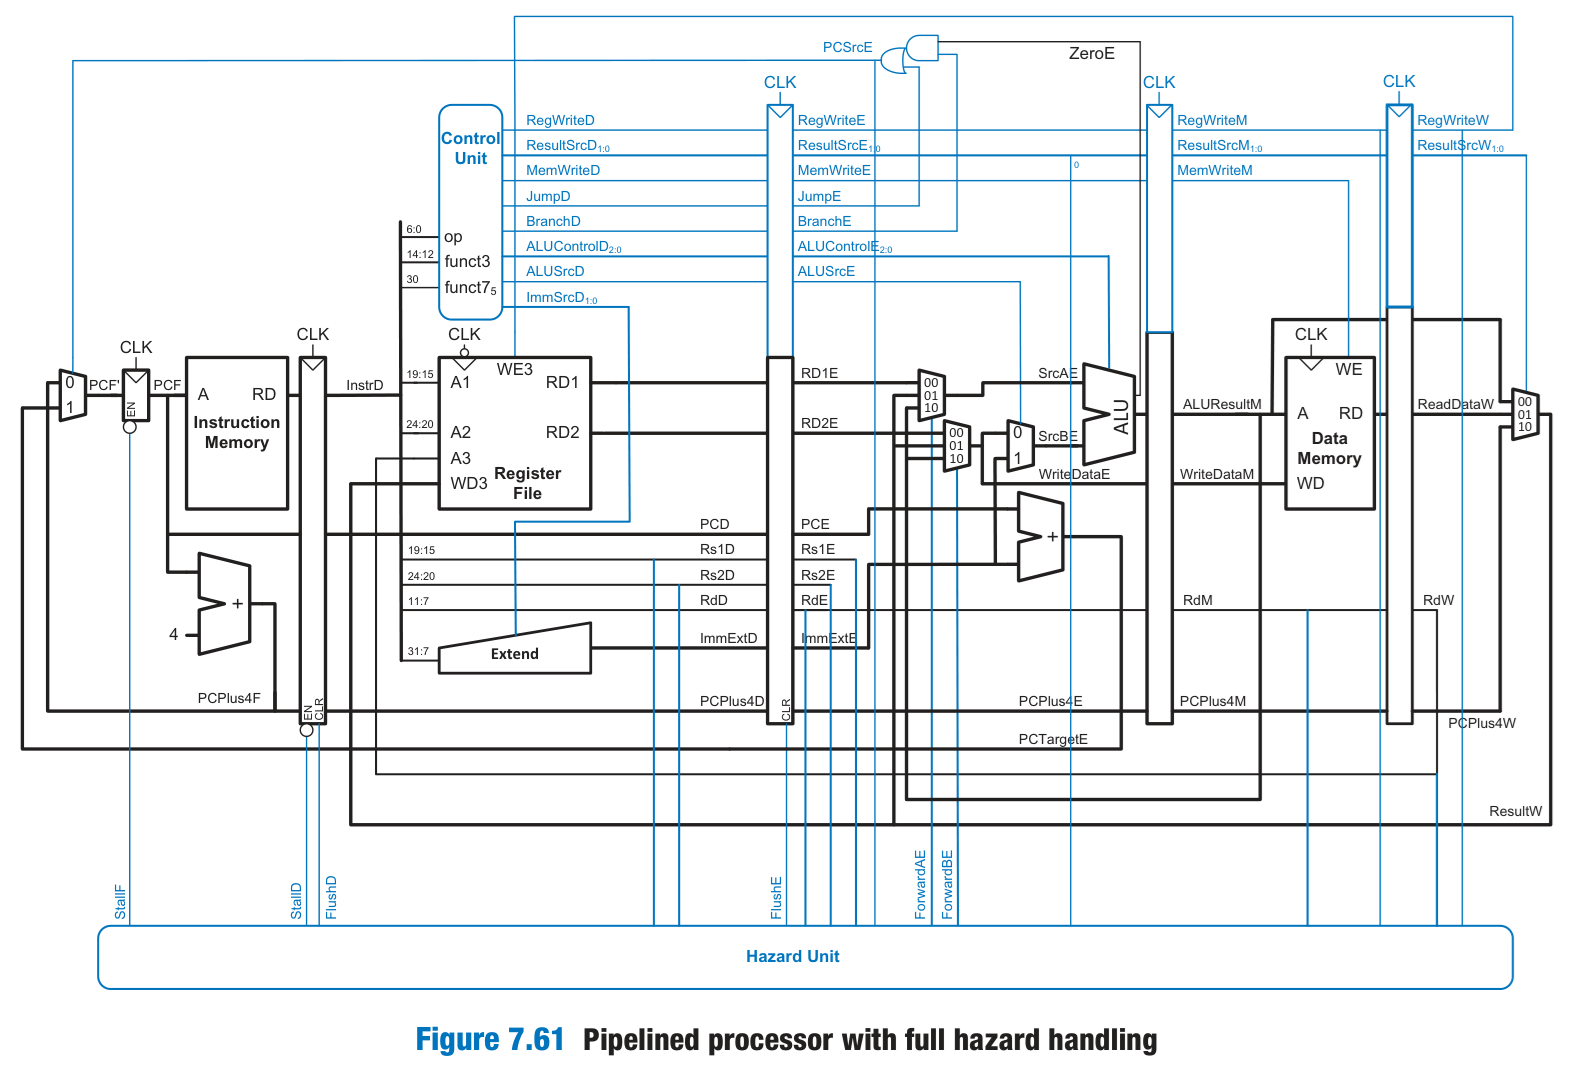
\includegraphics[width=\linewidth,height=0.78\textheight,keepaspectratio]{pipeline-processor.png}
    \column{0.38\textwidth}
    \small
    \begin{itemize}
      \item Cinco etapas con registros de pipeline IF/ID, ID/EX, EX/MEM, MEM/WB.
      \item \textbf{Hazard Unit}:
      \begin{itemize}
        \item \emph{Forwarding} desde MEM y WB hacia EX.
        \item \emph{Stall} de 1 ciclo por load-use.
        \item \emph{Flush} de 2 instrucciones por salto tomado (resuelto en EX).
      \end{itemize}
      \item Validado en E1 con 4 programas: ISA, forwarding, stalling y flushing.
      \item Límite: IPC $\le 1$.
    \end{itemize}
  \end{columns}
\end{frame}

\begin{frame}{Dual-Issue (B): organización}
  \begin{columns}[c]
    \column{0.58\textwidth}
    \centering\includegraphics[width=\linewidth,height=0.8\textheight,keepaspectratio]{dualissue-top.pdf}
    \column{0.4\textwidth}
    \small
    \begin{itemize}
      \item Fetch y Decode de \textbf{dos instrucciones consecutivas}: slot 0 (PC, más antigua) y slot 1 (PC+4).
      \item El slot 0 siempre va por la vía 0 y el slot 1 por la vía 1 $\Rightarrow$ el orden del programa se conserva en todas las etapas.
      \item Módulos nuevos: \sig{issue.v}, \sig{branchunit.v}, \sig{mux5.v}.
      \item Modificados: \sig{datapath}, \sig{controller}, \sig{hazard}, \sig{riscv}, \sig{imem}.
      \item Controller: un decodificador por vía; la decisión del salto pasa a la Branch Unit.
    \end{itemize}
  \end{columns}
\end{frame}

\begin{frame}{Dual-Issue (B): datapath completo}
  \begin{columns}[c]
    \column{0.72\textwidth}
    \centering\includegraphics[width=\linewidth,height=0.84\textheight,keepaspectratio]{dualissue-processor.pdf}
    \column{0.27\textwidth}
    \footnotesize
    \textbf{Por etapa}
    \begin{itemize}
      \item \textbf{IF}: \sig{RAM[PC]}, \sig{RAM[PC+4]}; PC $+8$, $+4$ o destino.
      \item \textbf{ID}: RF de 4 lecturas; reagrupamiento en IF/ID.
      \item \textbf{EX}: 2 ALU, forwarding \sig{mux5}, \textbf{1 Branch Unit}.
      \item \textbf{MEM}: \textbf{1 puerto}, \sig{MemLaneM} elige la vía.
      \item \textbf{WB}: 2 escrituras; si coinciden, gana la vía 1 (más joven).
    \end{itemize}
  \end{columns}
\end{frame}

\begin{frame}{Issue Unit: ¿dos, una o ninguna?}
  \small
  Combinacional sobre el par en Decode; solo considera los registros que cada instrucción \emph{realmente} lee.
  \vspace{0.2cm}

  \begin{tabularx}{\linewidth}{@{}lXl@{}}
    \toprule
    \textbf{Señal} & \textbf{Condición} & \textbf{Efecto}\\
    \midrule
    \sig{rawD} & El slot 0 escribe un registro ($\neq$ x0) que lee el slot 1 (no se puede adelantar en el mismo ciclo) & solo slot 0\\
    \sig{memD} & Ambas son \texttt{lw}/\texttt{sw}: un único puerto de memoria & solo slot 0\\
    \sig{ctrlD} & Ambas son \texttt{beq}/\texttt{jal}: una única Branch Unit & solo slot 0\\
    \sig{luseD\_1} & El slot 1 lee el destino de un \texttt{lw} que está en EX & solo slot 0\\
    \sig{LoadUseD\_0} & El slot 0 lee el destino de un \texttt{lw} que está en EX & \textbf{stall}\\
    \bottomrule
  \end{tabularx}
  \vspace{0.3cm}

  \begin{columns}[T]
    \column{0.5\textwidth}
    \clave{\centering $\sig{IssueOneD} = \sig{rawD} \lor \sig{memD} \lor \sig{ctrlD} \lor \sig{luseD\_1}$}
    \column{0.48\textwidth}
    \begin{itemize}\footnotesize
      \item Nunca se emite el slot 1 sin el slot 0 $\Rightarrow$ orden de programa.
      \item Recursos asignados a la vía que los necesita: ALU + \texttt{lw} y \texttt{lw} + ALU se emiten juntos.
      \item WAW/WAR dentro del par no se restringen: la vía 1 escribe después.
    \end{itemize}
  \end{columns}
\end{frame}

\begin{frame}{Emisión parcial y reagrupamiento}
  \begin{columns}[c]
    \column{0.55\textwidth}
    \centering\includegraphics[width=\linewidth]{pd-regroup.pdf}\par
    \nota{\texttt{sw x1} depende de \texttt{addi x1}: sale solo el slot 0 y el \texttt{sw} se reagrupa con la siguiente instrucción.}
    \column{0.43\textwidth}
    \small
    Si \sig{IssueOneD}$=1$, \sig{RegroupD} hace en el mismo flanco:
    \begin{enumerate}
      \item \sig{FlushE\_1}: el slot 1 no entra a EX (burbuja en la vía 1).
      \item IF/ID carga el slot 1 como nuevo slot 0 e \sig{InstrF\_0} como nuevo slot 1.
      \item El PC avanza \textbf{4} en lugar de 8.
    \end{enumerate}
    \medskip
    \clave{\small El nuevo par sigue siendo de dos instrucciones consecutivas: ninguna se pierde ni se repite, y la que esperaba puede salir en pareja en el ciclo siguiente.}
  \end{columns}
\end{frame}

\begin{frame}{Forwarding entre vías y stalls por load-use}
  \begin{columns}[T]
    \column{0.5\textwidth}
    \textbf{Forwarding} \nota{(4 operandos $\times$ 4 productores)}\par\smallskip
    \small Prioridad por antigüedad del productor:
    \[\text{MEM1} \succ \text{MEM0} \succ \text{WB1} \succ \text{WB0} \succ \text{RF}\]
    MEM es más reciente que WB y, en la misma etapa, la vía 1 es más joven: siempre se adelanta el valor más nuevo.\par\medskip
    \centering\includegraphics[width=0.95\linewidth]{pd-raw.pdf}
    \column{0.48\textwidth}
    \textbf{Load-use}\par\smallskip
    \small
    \begin{align*}
      \sig{lwStallD} &= \sig{LoadUseD\_0} \land \lnot\sig{PCSrcE}\\
      \sig{StallF} = \sig{StallD} &= \sig{lwStallD}\\
      \sig{FlushE\_0},\sig{FlushE\_1} &\leftarrow \sig{lwStallD}
    \end{align*}
    El dato del \texttt{lw} llega por WB0/WB1 un ciclo después. Load-use en el slot 1: basta con emitir solo el slot 0 (sin stall).\par\medskip
    \centering\includegraphics[width=0.95\linewidth]{pd-loaduse.pdf}
  \end{columns}
\end{frame}

\begin{frame}{Branches y flushing selectivo}
  \begin{columns}[T]
    \column{0.52\textwidth}
    \small
    Una sola Branch Unit; \sig{BrLaneE} elige los operandos de la vía con el salto.
    \[\sig{PCSrcE} = (\sig{BranchE}\land \sig{SrcAE}{=}\sig{SrcBE}) \lor \sig{JumpE}\]
    Salto tomado: se anulan solo las \textbf{más jóvenes}:
    \begin{itemize}
      \item IF/ID y ID/EX completos (\sig{FlushD}, \sig{FlushE\_0/1}).
      \item Salto en la vía 0: también su compañero de la vía 1 (\sig{FlushM\_1}).
      \item Salto en la vía 1: la vía 0 es más antigua y \textbf{se conserva}.
    \end{itemize}
    \column{0.46\textwidth}
    \footnotesize
    \begin{tabular}{@{}ll@{}}
      \toprule
      \textbf{Señal} & \textbf{Expresión}\\
      \midrule
      \sig{StallF/D} & \sig{LoadUseD\_0} $\land\lnot$\sig{PCSrcE}\\
      \sig{RegroupD} & \sig{IssueOneD} $\land\lnot$\sig{lwStallD} $\land\lnot$\sig{PCSrcE}\\
      \sig{FlushD} & \sig{PCSrcE}\\
      \sig{FlushE\_0} & \sig{lwStallD} $\lor$ \sig{PCSrcE}\\
      \sig{FlushE\_1} & \sig{lwStallD} $\lor$ \sig{PCSrcE} $\lor$ \sig{IssueOneD}\\
      \sig{FlushM\_1} & \sig{TakenE\_0}\\
      \bottomrule
    \end{tabular}
  \end{columns}
  \vspace{0.1cm}
  \centering\includegraphics[height=0.25\textheight]{pd-branch.pdf}
\end{frame}

\begin{frame}{Demo: doble emisión, RAW y reagrupamiento}
  \begin{columns}[c]
    \column{0.6\textwidth}
    \centering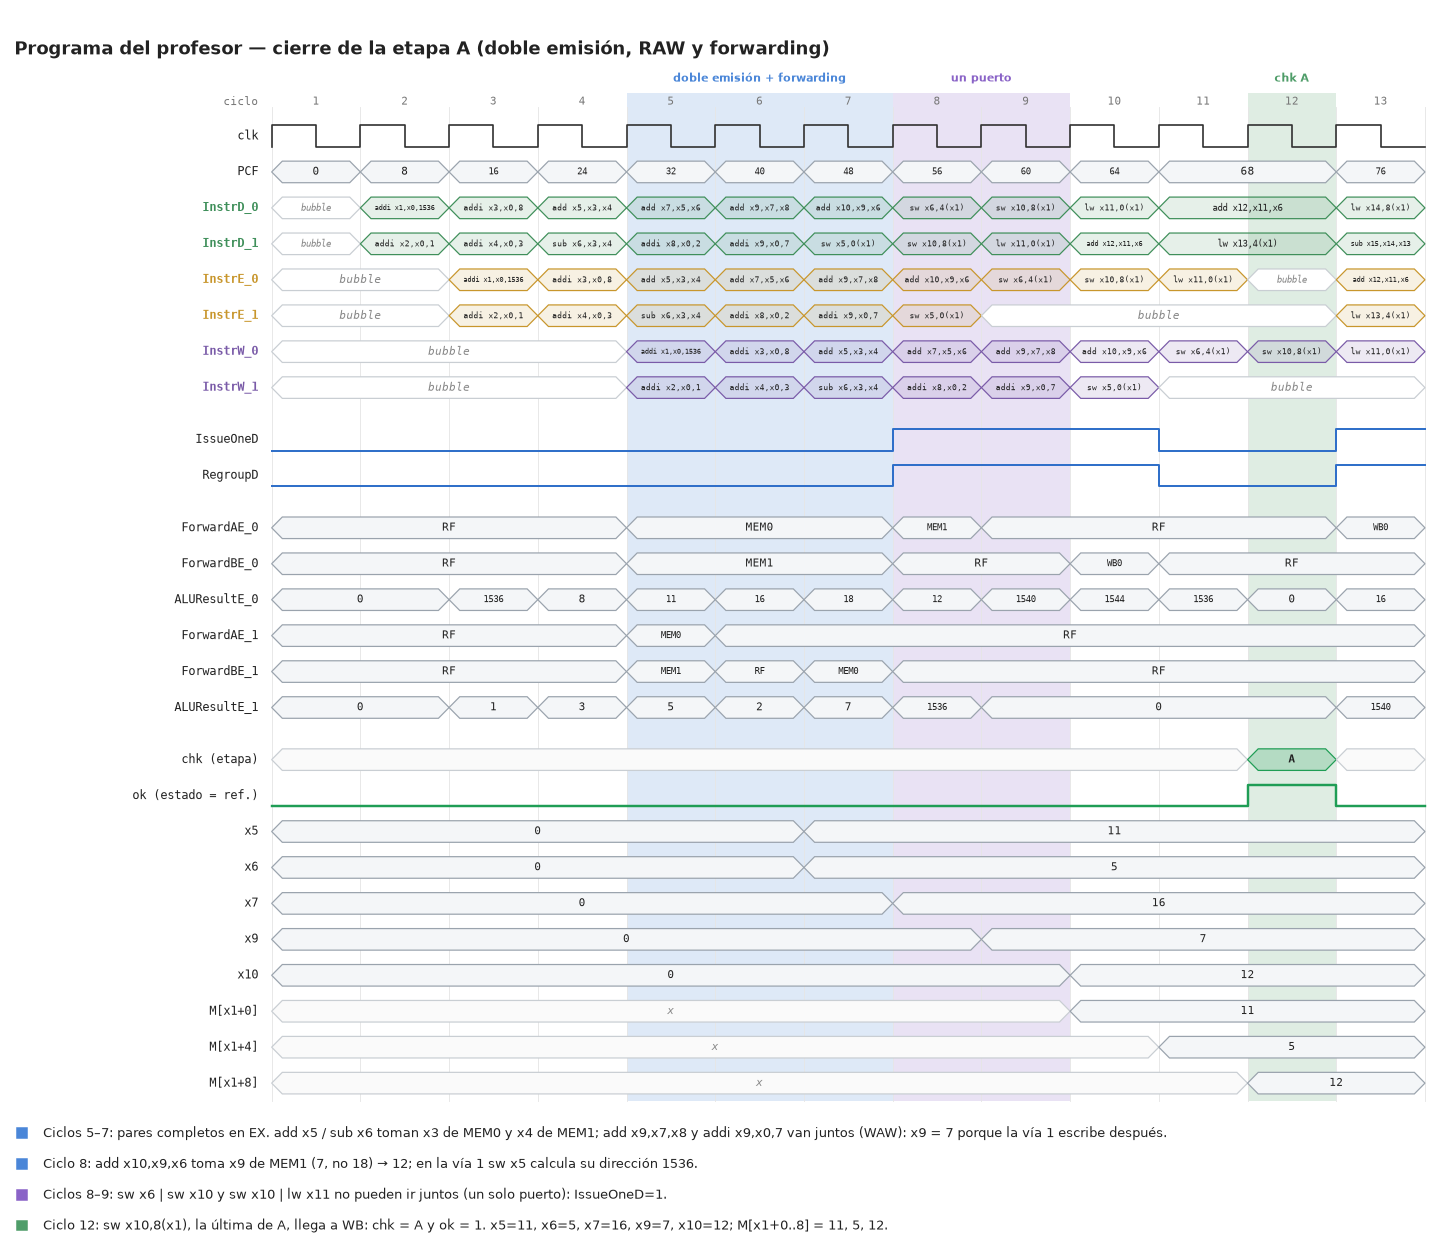
\includegraphics[width=\linewidth,height=0.84\textheight,keepaspectratio]{waveform-prog-A.png}
    \column{0.39\textwidth}
    \scriptsize
    Programa del profesor, etapa A (arquitectura C):
    \begin{itemize}
      \item \textbf{Ciclos 5--7}: pares completos en EX. \texttt{add x5} y \texttt{sub x6} toman x3 de MEM0 y x4 de MEM1.
      \item \texttt{add x9,x7,x8} y \texttt{addi x9,x0,7} van juntos (WAW): x9$=7$ porque la vía 1 escribe después.
      \item \textbf{Ciclos 8--9}: dos \texttt{sw} seguidos no caben juntos (un puerto): \sig{IssueOneD}$=1$ y \sig{RegroupD}$=1$.
      \item \textbf{Ciclo 12}: \texttt{sw x10,8(x1)} llega a WB, \sig{chk}$=$A, \sig{ok}$=1$: x5$=11$, x6$=5$, x7$=16$, x9$=7$, x10$=12$, M[x1+0..8]$=$11, 5, 12.
    \end{itemize}
  \end{columns}
\end{frame}

\begin{frame}{Demo: load-use y un solo puerto de memoria}
  \begin{columns}[c]
    \column{0.64\textwidth}
    \centering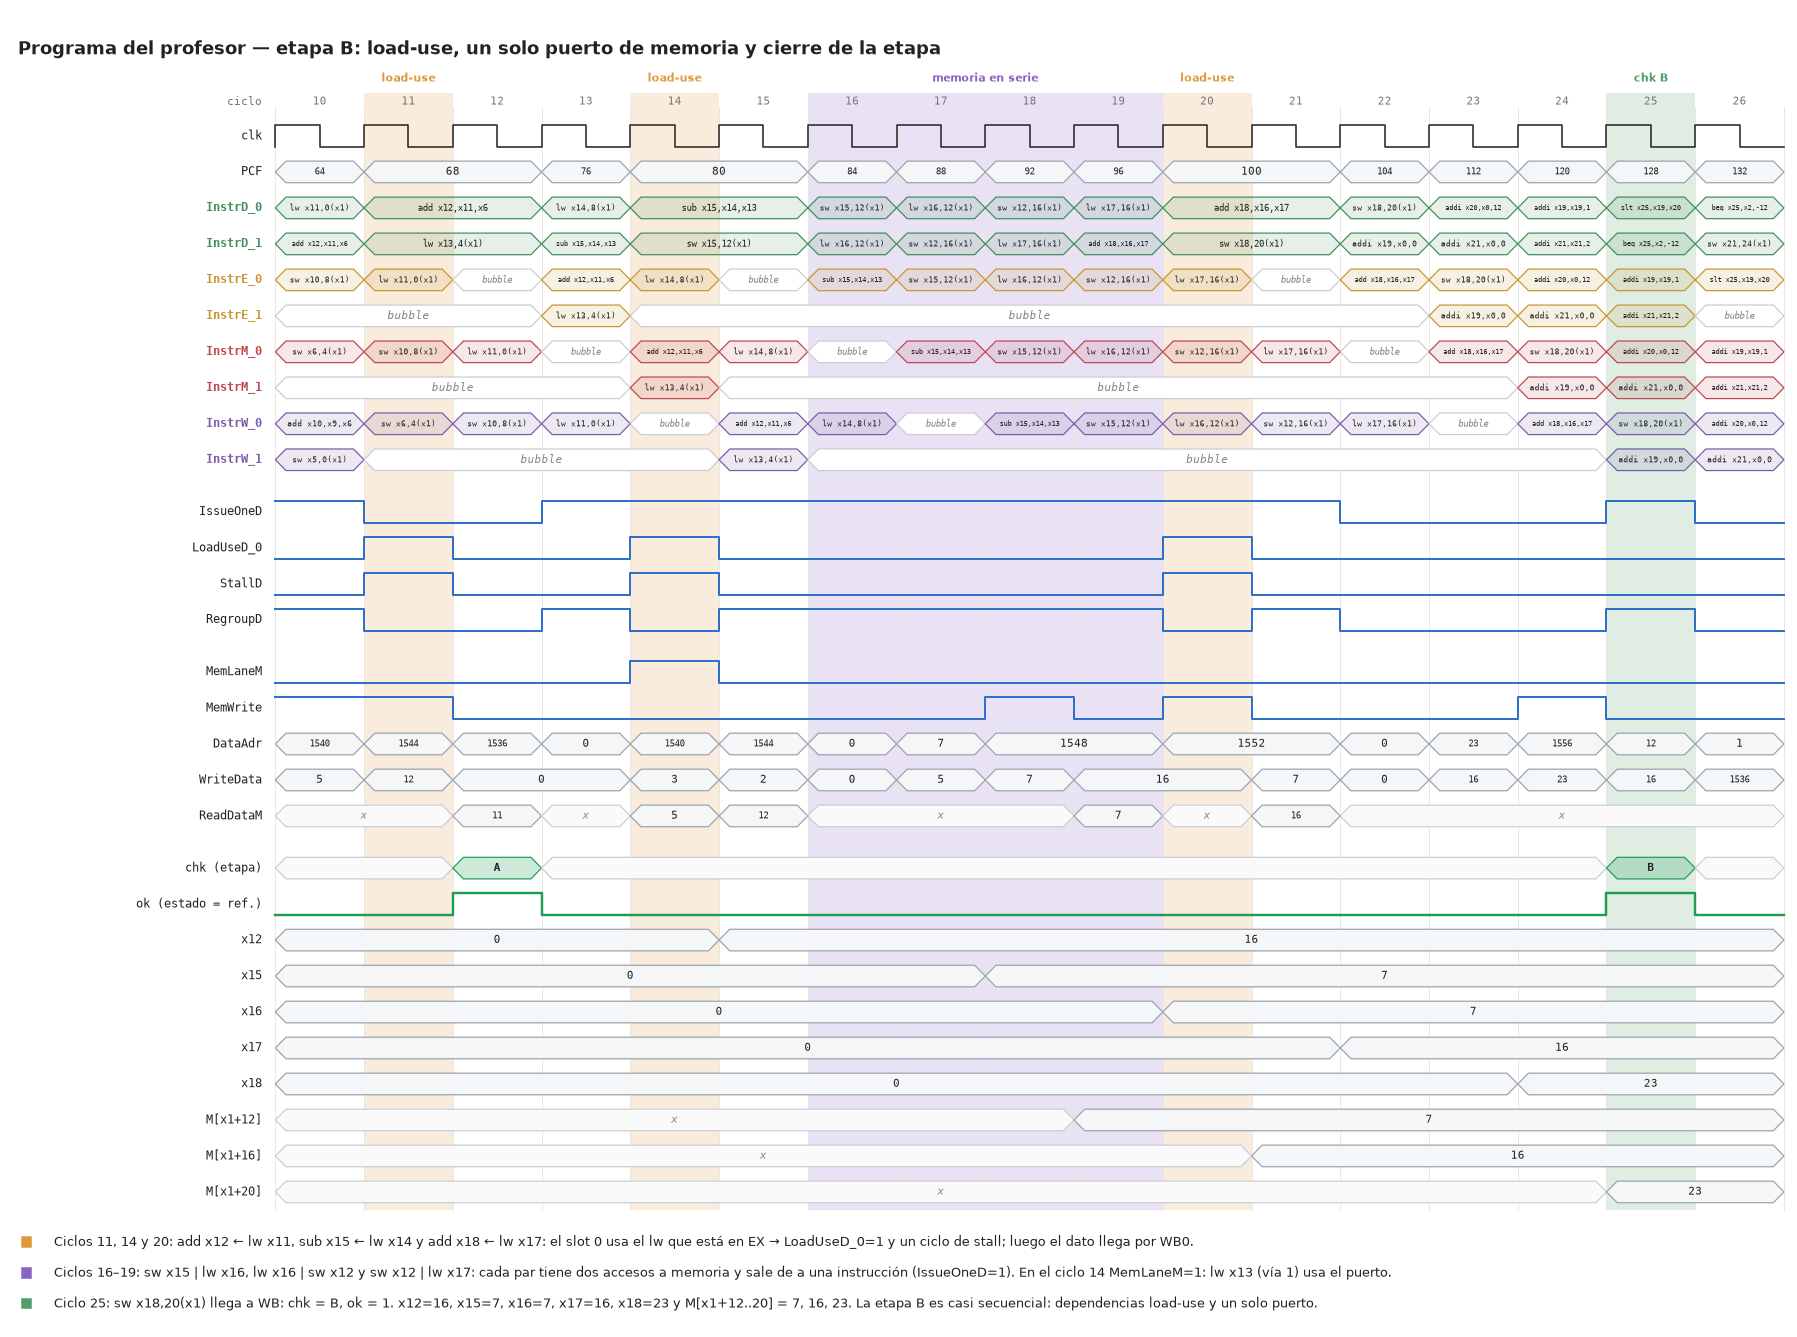
\includegraphics[width=\linewidth,height=0.84\textheight,keepaspectratio]{waveform-prog-B.png}
    \column{0.35\textwidth}
    \scriptsize
    Programa del profesor, etapa B:
    \begin{itemize}
      \item \textbf{Load-use} (ciclos 11, 14, 20): el consumidor del \texttt{lw} espera un ciclo; \sig{StallF}/\sig{StallD} y burbujas en EX.
      \item \textbf{Memoria en serie} (ciclos 16--19): \texttt{lw}/\texttt{sw} consecutivos nunca se emiten juntos.
      \item El dato llega por \textbf{WB0/WB1}.
      \item \textbf{Ciclo 25}: cierre de B, \sig{ok}$=1$ (x15$=7$, x18$=23$, M[x1+12..20]$=$7, 16, 23).
    \end{itemize}
  \end{columns}
\end{frame}

% =====================================================================
\section{Optimización: predicción dinámica de saltos}

\begin{frame}{Motivación: el costo de los saltos tomados en B}
  \begin{columns}[c]
    \column{0.55\textwidth}
    \centering\includegraphics[width=\linewidth]{pd-nopred.pdf}\par
    \nota{B: el \texttt{beq} tomado descarta su compañero y dos pares. 5 ciclos por iteración, solo 3 útiles.}
    \column{0.43\textwidth}
    \small
    \begin{itemize}
      \item B resuelve el salto en EX y Fetch sigue en secuencia: predice siempre \emph{no tomado}.
      \item Cada salto tomado cuesta \textbf{2 ciclos} y hasta \textbf{4 instrucciones} (en A, 2).
      \item La Issue Unit no puede resolverlo: Fetch no sabe a dónde ir.
    \end{itemize}
    \medskip
    \footnotesize
    \begin{tabular}{@{}lccc@{}}
      \toprule
      \textbf{Programa (B)} & \textbf{Tomados} & \textbf{Flush} & \textbf{\%}\\
      \midrule
      Profesor & 68 & 136 / 387 & 35\,\%\\
      Propio & 199 & 398 / 1421 & 28\,\%\\
      \bottomrule
    \end{tabular}
  \end{columns}
\end{frame}

\begin{frame}{Propuesta: BTB con contador saturado de 2 bits}
  \begin{columns}[T]
    \column{0.5\textwidth}
    \small
    \begin{itemize}
      \item El BTB se consulta en Fetch con los PC de \textbf{ambos slots}.
      \item Si hay acierto y el contador predice tomado, el PC siguiente es el destino guardado, sin esperar a EX.
      \item La Branch Unit ahora \textbf{verifica} la predicción: solo se descarta si falla.
      \item \textbf{BTB}: Fetch aún no sabe si la instrucción es un salto ni su destino; solo tiene el PC.
      \item \textbf{2 bits} vs 1 bit: en un bucle, 1 bit falla dos veces por ejecución; 2 bits solo a la salida.
    \end{itemize}
    \column{0.48\textwidth}
    \centering\includegraphics[width=\linewidth]{fsm-2bit.pdf}\par
    \nota{Predicción $=$ \sig{Ctr[1]}. Un \texttt{beq} entra en \texttt{10}; un \texttt{jal} directamente en \texttt{11}.}
    \vspace{0.3cm}
    \footnotesize
    \begin{tabularx}{\linewidth}{@{}lX@{}}
      \toprule
      Limitación & 2 ciclos por salto tomado\\
      Módulos & \sig{btb.v} (nuevo), \sig{datapath}, \sig{branchunit}, \sig{hazard}, \sig{riscv}\\
      Métricas & ciclos, IPC, CPI, speedup, errores, precisión, aciertos BTB\\
      \bottomrule
    \end{tabularx}
  \end{columns}
\end{frame}

\begin{frame}{Branch Target Buffer}
  \begin{columns}[c]
    \column{0.55\textwidth}
    \centering\includegraphics[width=\linewidth,height=0.75\textheight,keepaspectratio]{btb-inside.pdf}
    \column{0.43\textwidth}
    \footnotesize
    \begin{itemize}
      \item 16 entradas, correspondencia directa, índice \sig{PC[5:2]}.
      \item Entrada: V (1) + Tag \sig{PC[31:6]} (26) + Ctr (2) + destino (32) $=$ 61 bits; \textbf{976 bits} en total.
      \item 2 puertos de lectura combinacionales (\sig{PCF}, \sig{PCPlus4F}), 1 de escritura desde EX.
    \end{itemize}
    \clave{\centering $\sig{predtaken} = \sig{V} \land (\sig{Tag} = \sig{PC[31:6]}) \land \sig{Ctr[1]}$}
    \medskip
    \footnotesize
    \begin{itemize}
      \item Tomado: escribe V, Tag, destino y contador. No tomado con acierto: decrementa.
      \item Se actualiza con el contador \emph{actual} de la tabla, no con una copia de Fetch.
    \end{itemize}
  \end{columns}
\end{frame}

\begin{frame}{Fetch con predicción}
  \begin{columns}[c]
    \column{0.36\textwidth}
    \centering\includegraphics[width=\linewidth,height=0.84\textheight,keepaspectratio]{proc-btb-zoom-fetch.pdf}
    \column{0.62\textwidth}
    \small
    Cadena de multiplexores con prioridad:
    \[
    \sig{PCNextF} =
    \begin{cases}
      \sig{PCCorrectE} & \sig{MispredictE}\ \text{(error en EX)}\\
      \sig{TargetF\_0} & \sig{PredF\_0}\ \text{(slot 0 predicho)}\\
      \sig{PCPlus4F} & \sig{RegroupD}\ \text{(emisión parcial)}\\
      \sig{TargetF\_1} & \sig{PredF\_1}\ \text{(slot 1 predicho)}\\
      \sig{PCPlus8F} & \text{otro caso}
    \end{cases}
    \]
    \begin{itemize}\footnotesize
      \item \sig{PredF\_0} antes que \sig{RegroupD}: al reagrupar, \sig{InstrF\_0} pasa al slot 1 y lo que le sigue es su destino.
      \item \sig{RegroupD} antes que \sig{PredF\_1}: \sig{InstrF\_1} se descarta y se vuelve a buscar.
      \item Slot 0 predicho tomado: el slot 1 está fuera del camino:\\
        \alert{$\sig{AnnulF\_1} = \sig{PredF\_0} \land \lnot\sig{RegroupD}$}
      \item \{Pred, Target\} viajan con la instrucción (33 bits): obedecen los mismos stalls, flushes y reagrupamientos.
    \end{itemize}
  \end{columns}
\end{frame}

\begin{frame}{Verificación en la Branch Unit y Hazard Unit}
  \begin{columns}[c]
    \column{0.5\textwidth}
    \centering\includegraphics[width=\linewidth,height=0.46\textheight,keepaspectratio]{bu-inside.pdf}
    \scriptsize
    \begin{align*}
      \sig{MispredictE} &= \sig{CtrlE} \land \bigl[(\sig{PCSrcE} \neq \sig{PredTakenE})\\
        &\quad\lor (\sig{PCSrcE} \land \sig{PCTargetE} \neq \sig{PredTargetE})\bigr]\\
      \sig{PCCorrectE} &= \sig{PCSrcE}\ ?\ \sig{PCTargetE} : \sig{PCPlus4E}\\
      \sig{FlushLane1E} &= \sig{MispredictE} \land \lnot\sig{BrLaneE}
    \end{align*}
    \column{0.48\textwidth}
    \small
    La Hazard Unit \textbf{conserva su estructura}: se anula por \emph{error de predicción} y no por \emph{salto tomado}.\par\medskip
    \scriptsize
    \begin{tabular}{@{}lll@{}}
      \toprule
      \textbf{Señal} & \textbf{B} & \textbf{C}\\
      \midrule
      \sig{FlushD} & \sig{PCSrcE} & \alert{\sig{MispredictE}}\\
      \sig{FlushE\_0} & \sig{lwStallD} $\lor$ \sig{PCSrcE} & \sig{lwStallD} $\lor$ \alert{\sig{MispredictE}}\\
      \sig{FlushM\_1} & \sig{TakenE\_0} & \alert{\sig{FlushLane1E}}\\
      \sig{lwStallD} & \ldots$\land\lnot$\sig{PCSrcE} & \ldots$\land\lnot$\alert{\sig{MispredictE}}\\
      \sig{RegroupD} & \ldots$\land\lnot$\sig{PCSrcE} & \ldots$\land\lnot$\alert{\sig{MispredictE}}\\
      \bottomrule
    \end{tabular}\par\medskip
    \small Caso nuevo: predicho tomado que no se toma $\Rightarrow$ volver a \sig{PC}+4 del salto (la Branch Unit recibe \sig{PCPlus4E} de cada vía).
  \end{columns}
\end{frame}

\begin{frame}{Datapath de C: Dual-Issue con predicción}
  \begin{columns}[c]
    \column{0.72\textwidth}
    \centering\includegraphics[width=\linewidth,height=0.84\textheight,keepaspectratio]{proc-btb.pdf}
    \column{0.27\textwidth}
    \scriptsize
    En \textcolor{opt}{\textbf{café}} lo nuevo:
    \begin{itemize}
      \item BTB en Fetch
      \item Cadena del PC siguiente
      \item Reagrupamiento y anulación de la predicción
      \item \{Pred, Target\} hasta la Branch Unit
      \item \sig{PCCorrectE} y actualización del BTB
    \end{itemize}
    \medskip
    \textbf{Costo}: 976 bits de BTB + 132 bits de registros de pipeline, 2 comparadores de 26 bits, 1 de 32 bits, 7 mux 2:1.\par
    \nota{Issue Unit, forwarding, RF, memoria y Controller: sin cambios.}
  \end{columns}
\end{frame}

\begin{frame}{Demo: salto predicho en el slot 0}
  \begin{columns}[c]
    \column{0.64\textwidth}
    \centering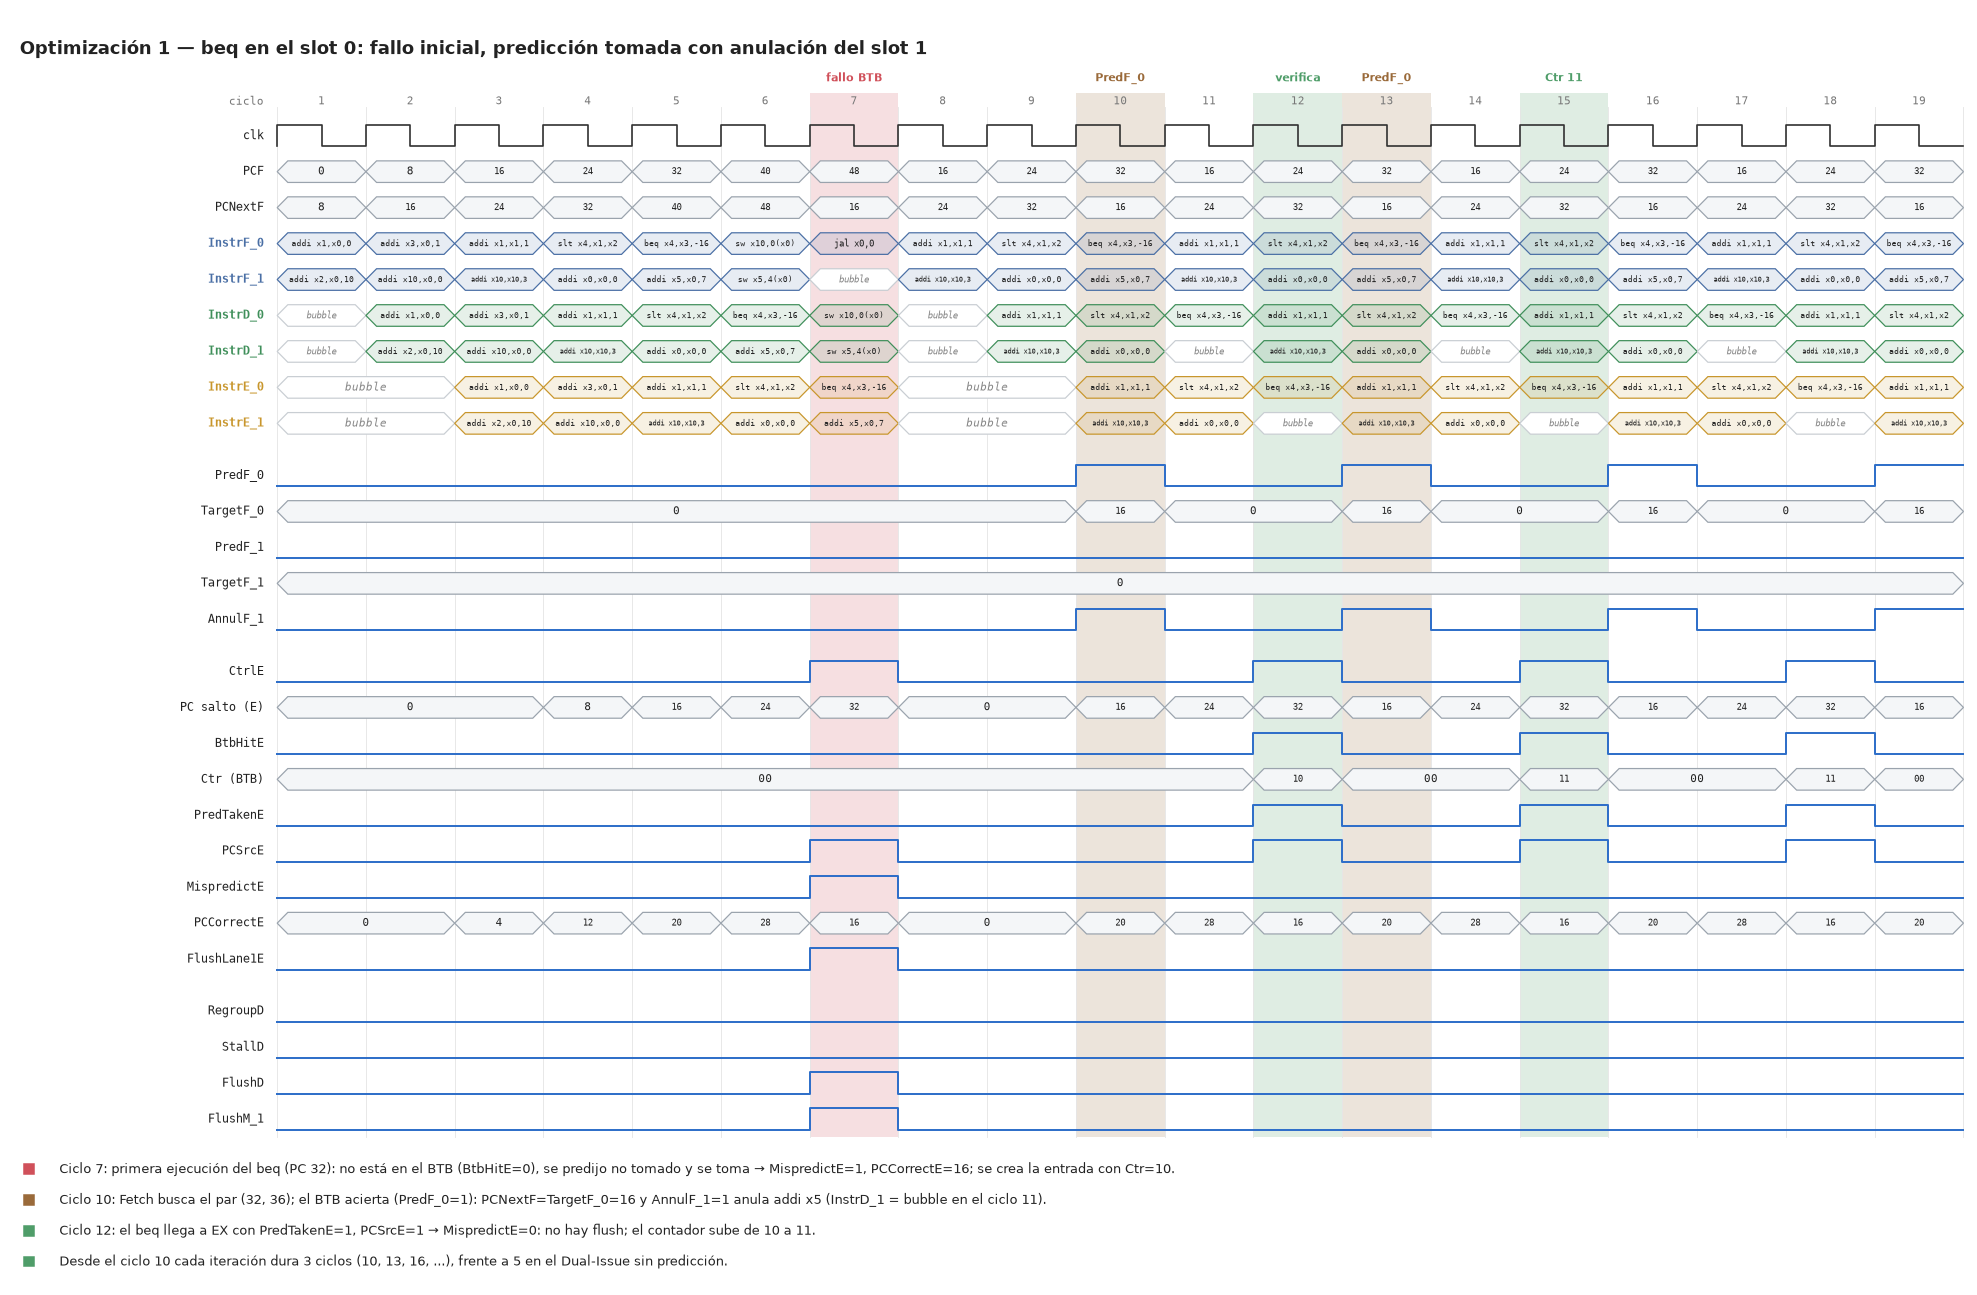
\includegraphics[width=\linewidth,height=0.84\textheight,keepaspectratio]{waveform-opt-slot0.png}
    \column{0.35\textwidth}
    \scriptsize
    Prueba \texttt{pred\_slot0} en C:
    \begin{itemize}
      \item \textbf{Ciclo 7}: primera ejecución sin entrada (\sig{BtbHitE}$=0$): \sig{MispredictE}$=1$, igual que en B; se crea la entrada en \texttt{10}.
      \item \textbf{Ciclo 10}: \sig{PredF\_0}$=1$, \sig{PCNextF}$=16$ y \sig{AnnulF\_1}$=1$: \texttt{addi x5} no entra.
      \item \textbf{Ciclo 12}: se confirma, sin flush; el contador pasa a \texttt{11}.
      \item Iteración: \textbf{5 $\to$ 3 ciclos}. Errores 10 $\to$ 3, ciclos 56 $\to$ 42.
    \end{itemize}
    \centering\includegraphics[width=\linewidth,height=0.25\textheight,keepaspectratio]{pd-pred-slot0.pdf}
  \end{columns}
\end{frame}

\begin{frame}{Demo: slot 1 y salida del bucle}
  \begin{columns}[T]
    \column{0.5\textwidth}
    \centering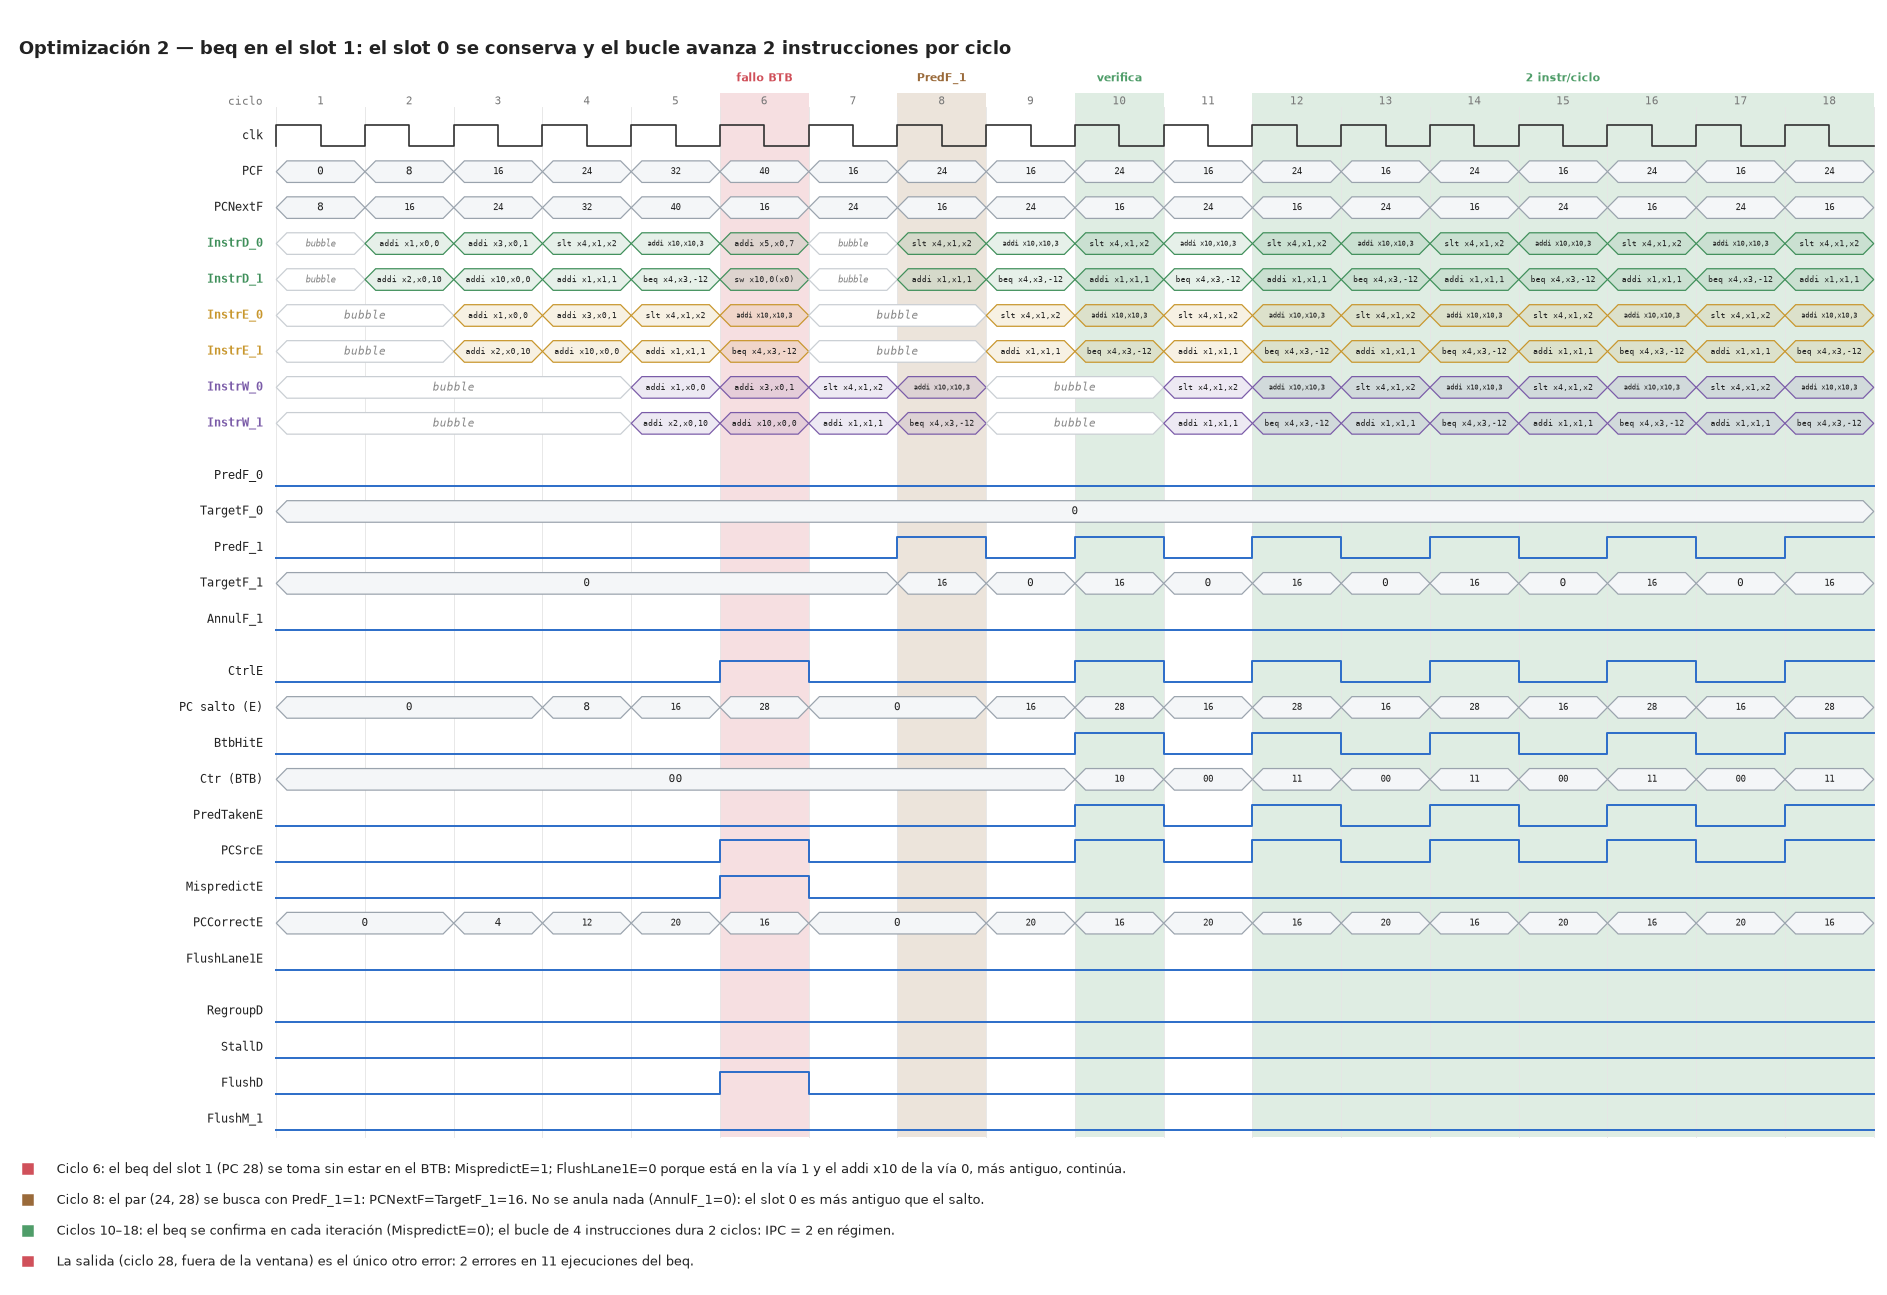
\includegraphics[width=\linewidth,height=0.6\textheight,keepaspectratio]{waveform-opt-slot1.png}\par
    \footnotesize\raggedright
    \textbf{Slot 1} (\texttt{pred\_slot1}): \sig{FlushLane1E}$=0$, la vía 0 más antigua continúa; \sig{PredF\_1}$=1$, \sig{AnnulF\_1}$=0$. Desde el ciclo 10, \textbf{2 instrucciones por ciclo}: 50 $\to$ 34 ciclos (speedup 1.47, IPC 1.53).
    \column{0.48\textwidth}
    \centering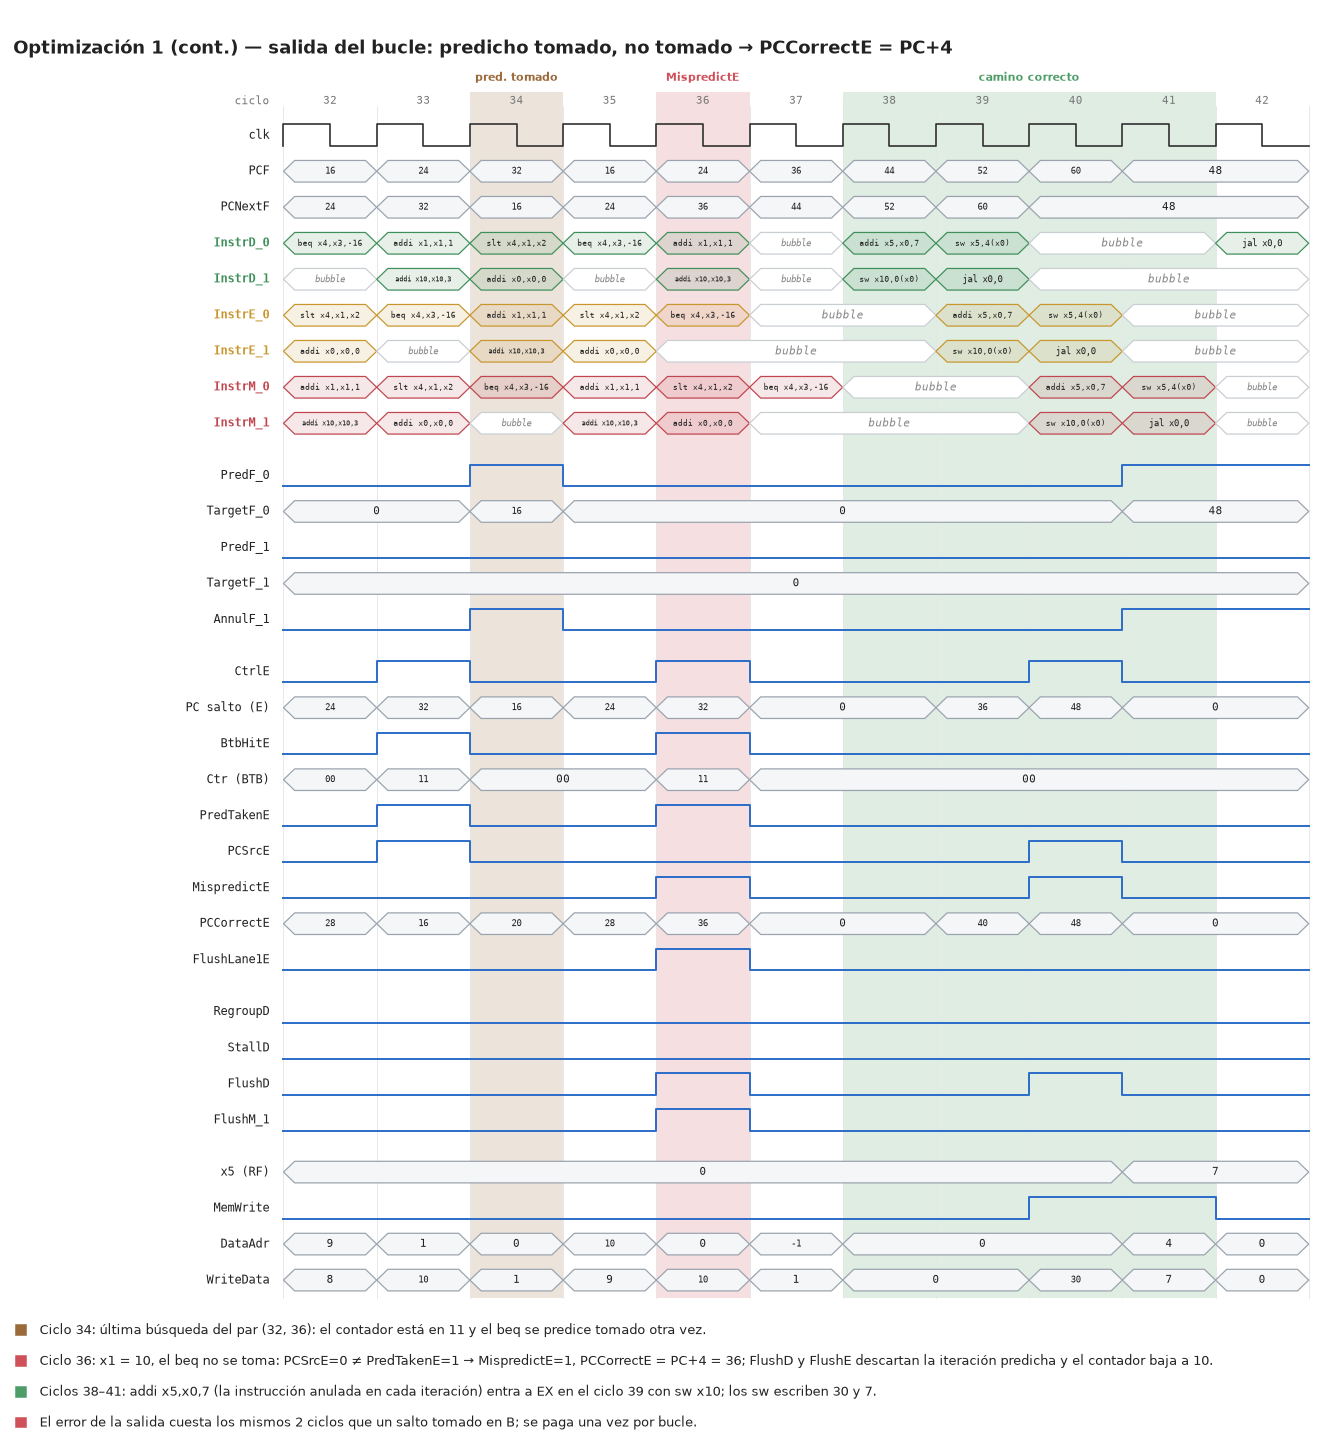
\includegraphics[width=\linewidth,height=0.6\textheight,keepaspectratio]{waveform-opt-slot0-exit.png}\par
    \footnotesize\raggedright
    \textbf{Salida}: el \texttt{beq} se predice tomado y no se toma: \sig{MispredictE}$=1$, Fetch retoma en \sig{PCCorrectE}$=$\sig{PCPlus4E}$=36$; el contador baja a \texttt{10}.
  \end{columns}
\end{frame}

\begin{frame}{Validación de la optimización}
  \small
  Siete programas específicos (\texttt{tb/programs/opt/}); en todos, el estado final de C coincide con el esperado y con A y B.
  \vspace{0.2cm}

  \footnotesize
  \begin{tabularx}{\linewidth}{@{}lXcc@{}}
    \toprule
    \textbf{Programa} & \textbf{Caso que verifica} & \textbf{Err. B} & \textbf{Err. C}\\
    \midrule
    \texttt{pred\_slot0} & Salto en el slot 0: anulación del slot 1, error a la salida y retorno a PC+4 & 10 & 3\\
    \texttt{pred\_slot1} & Salto en el slot 1: el slot 0, más antiguo, se conserva & 11 & 3\\
    \texttt{pred\_regroup} & Salto predicho que se reagrupa por RAW con la primera instrucción de su destino & 6 & 3\\
    \texttt{pred\_jal} & \texttt{jal} en el BTB (contador \texttt{11}) y salto hacia adelante tomado una vez & 12 & 4\\
    \texttt{pred\_pattern} & Patrón T, T, N: un error por periodo; el no tomado retoma en PC+4 & 15 & 7\\
    \texttt{pred\_loaduse} & Stall por load-use detrás de un salto bien predicho (caso nuevo) & 4 & 3\\
    \texttt{pred\_alias} & Dos saltos con el mismo índice: solo fallos, nunca un resultado incorrecto (Tag) & 15 & 15\\
    \bottomrule
  \end{tabularx}
  \vspace{0.3cm}

  \small
  \textbf{Infraestructura}: \texttt{tb/perf\_tb.v} (un testbench para A/B/C con \texttt{-DDUAL}, \texttt{-DOPT} y contadores de rendimiento), \texttt{tb/run\_all.sh} (compara registros y memoria de A, B y C), \texttt{final\_tb.v} (etapas del programa del profesor).
\end{frame}

% =====================================================================
\section{Programas y comparación}

\begin{frame}[fragile]{Programa propio: ordenamiento burbuja}
  \begin{columns}[T]
    \column{0.48\textwidth}
    \small
    \begin{enumerate}
      \item \textbf{Generación}: 16 números pseudoaleatorios, $x \leftarrow (5x+3) \bmod 64$.
      \item \textbf{Ordenamiento}: dos bucles anidados; compara $a[j]$ y $a[j+1]$ e intercambia.
      \item \textbf{Verificación}: suma del arreglo y conteo de inversiones (debe dar 0).
    \end{enumerate}
    \medskip
    \textbf{Por qué}: dos \texttt{lw} que compiten por el puerto de memoria, dependencias, un salto de bucle predecible y uno que depende de los datos (\texttt{noswap}).
    \column{0.5\textwidth}
    \footnotesize
\begin{verbatim}
inner:  lw   x13, 0(x12)    ; a[j]
        lw   x14, 4(x12)    ; a[j+1]
        addi x12, x12, 4
        slt  x16, x12, x11  ; j < end
        slt  x15, x14, x13  ; a[j+1] < a[j]
        beq  x15, x0, noswap
        sw   x14, -4(x12)
        sw   x13, 0(x12)
        addi x18, x18, 1
noswap: beq  x16, x3, inner
\end{verbatim}
    \clave{\footnotesize Arreglo ordenado, sin inversiones e idéntico en A, B y C.}
  \end{columns}
\end{frame}

\begin{frame}{Programa del profesor: comprobación de las etapas}
  \begin{columns}[T]
    \column{0.44\textwidth}
    \small
    \begin{itemize}
      \item Se ejecuta sin modificaciones en A, B y C.
      \item \textbf{A}: dependencias. \textbf{B}: memoria. \textbf{C}: bucles. \textbf{D}: integración.
      \item Al cerrar cada etapa, el testbench compara registros y memoria con la referencia.
    \end{itemize}
    \column{0.54\textwidth}
    \footnotesize
    \centering
    \setlength{\tabcolsep}{4pt}
    \begin{tabular}{@{}lcccccc@{}}
      \toprule
      & \multicolumn{2}{c}{\textbf{A}} & \multicolumn{2}{c}{\textbf{B}} & \multicolumn{2}{c}{\textbf{C}}\\
      \cmidrule(lr){2-3}\cmidrule(lr){4-5}\cmidrule(lr){6-7}
      \textbf{Etapa} & Ciclo & Estado & Ciclo & Estado & Ciclo & Estado\\
      \midrule
      A & 18 & \textcolor{good}{OK} & 12 & \textcolor{good}{OK} & 12 & \textcolor{good}{OK}\\
      B & 32 & \textcolor{good}{OK} & 25 & \textcolor{good}{OK} & 25 & \textcolor{good}{OK}\\
      C & 362 & \textcolor{good}{OK} & 312 & \textcolor{good}{OK} & 220 & \textcolor{good}{OK}\\
      D & 459 & \textcolor{good}{OK} & 387 & \textcolor{good}{OK} & 292 & \textcolor{good}{OK}\\
      \bottomrule
    \end{tabular}
  \end{columns}
  \vspace{0.4cm}
  \small
  \clave{Etapas A y B sin saltos: B y C empatan. La ganancia está en la etapa C (bucles); en D casi no hay, sus saltos se ejecutan una sola vez.}
  \vspace{0.2cm}
  \nota{Equivalencia: los 23 programas del proyecto dan el mismo estado en A, B y C.}
\end{frame}

\begin{frame}{Etapa C1: la predicción ayuda}
  \centering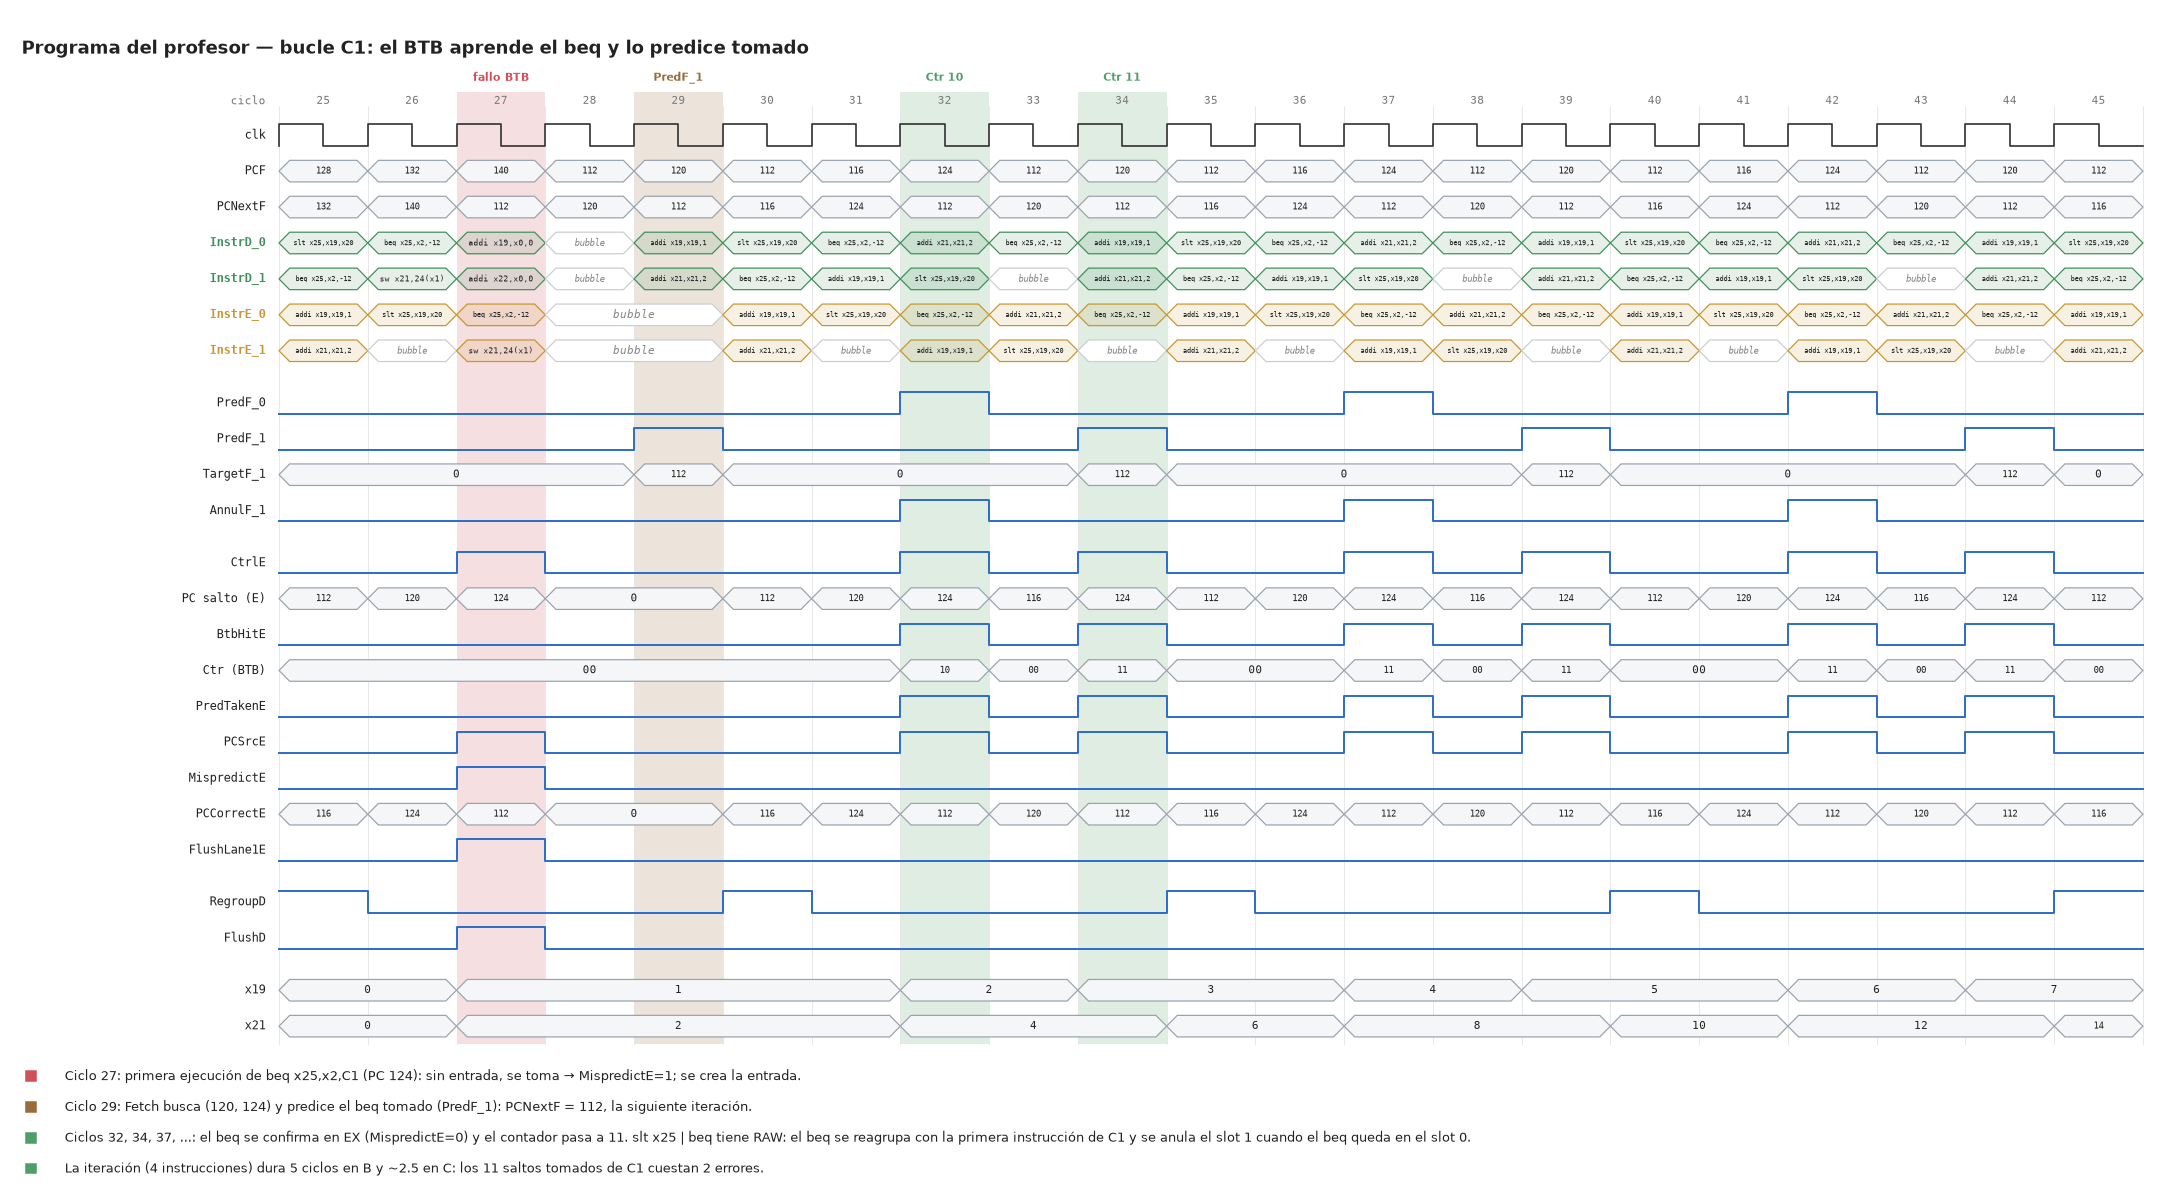
\includegraphics[width=\linewidth,height=0.72\textheight,keepaspectratio]{waveform-prog-C1.png}\par
  \vspace{0.2cm}\small El salto de cierre solo falla la primera vez y a la salida. Cada vuelta tarda la mitad.
\end{frame}

\begin{frame}{Etapa C2: la predicción no ayuda}
  \centering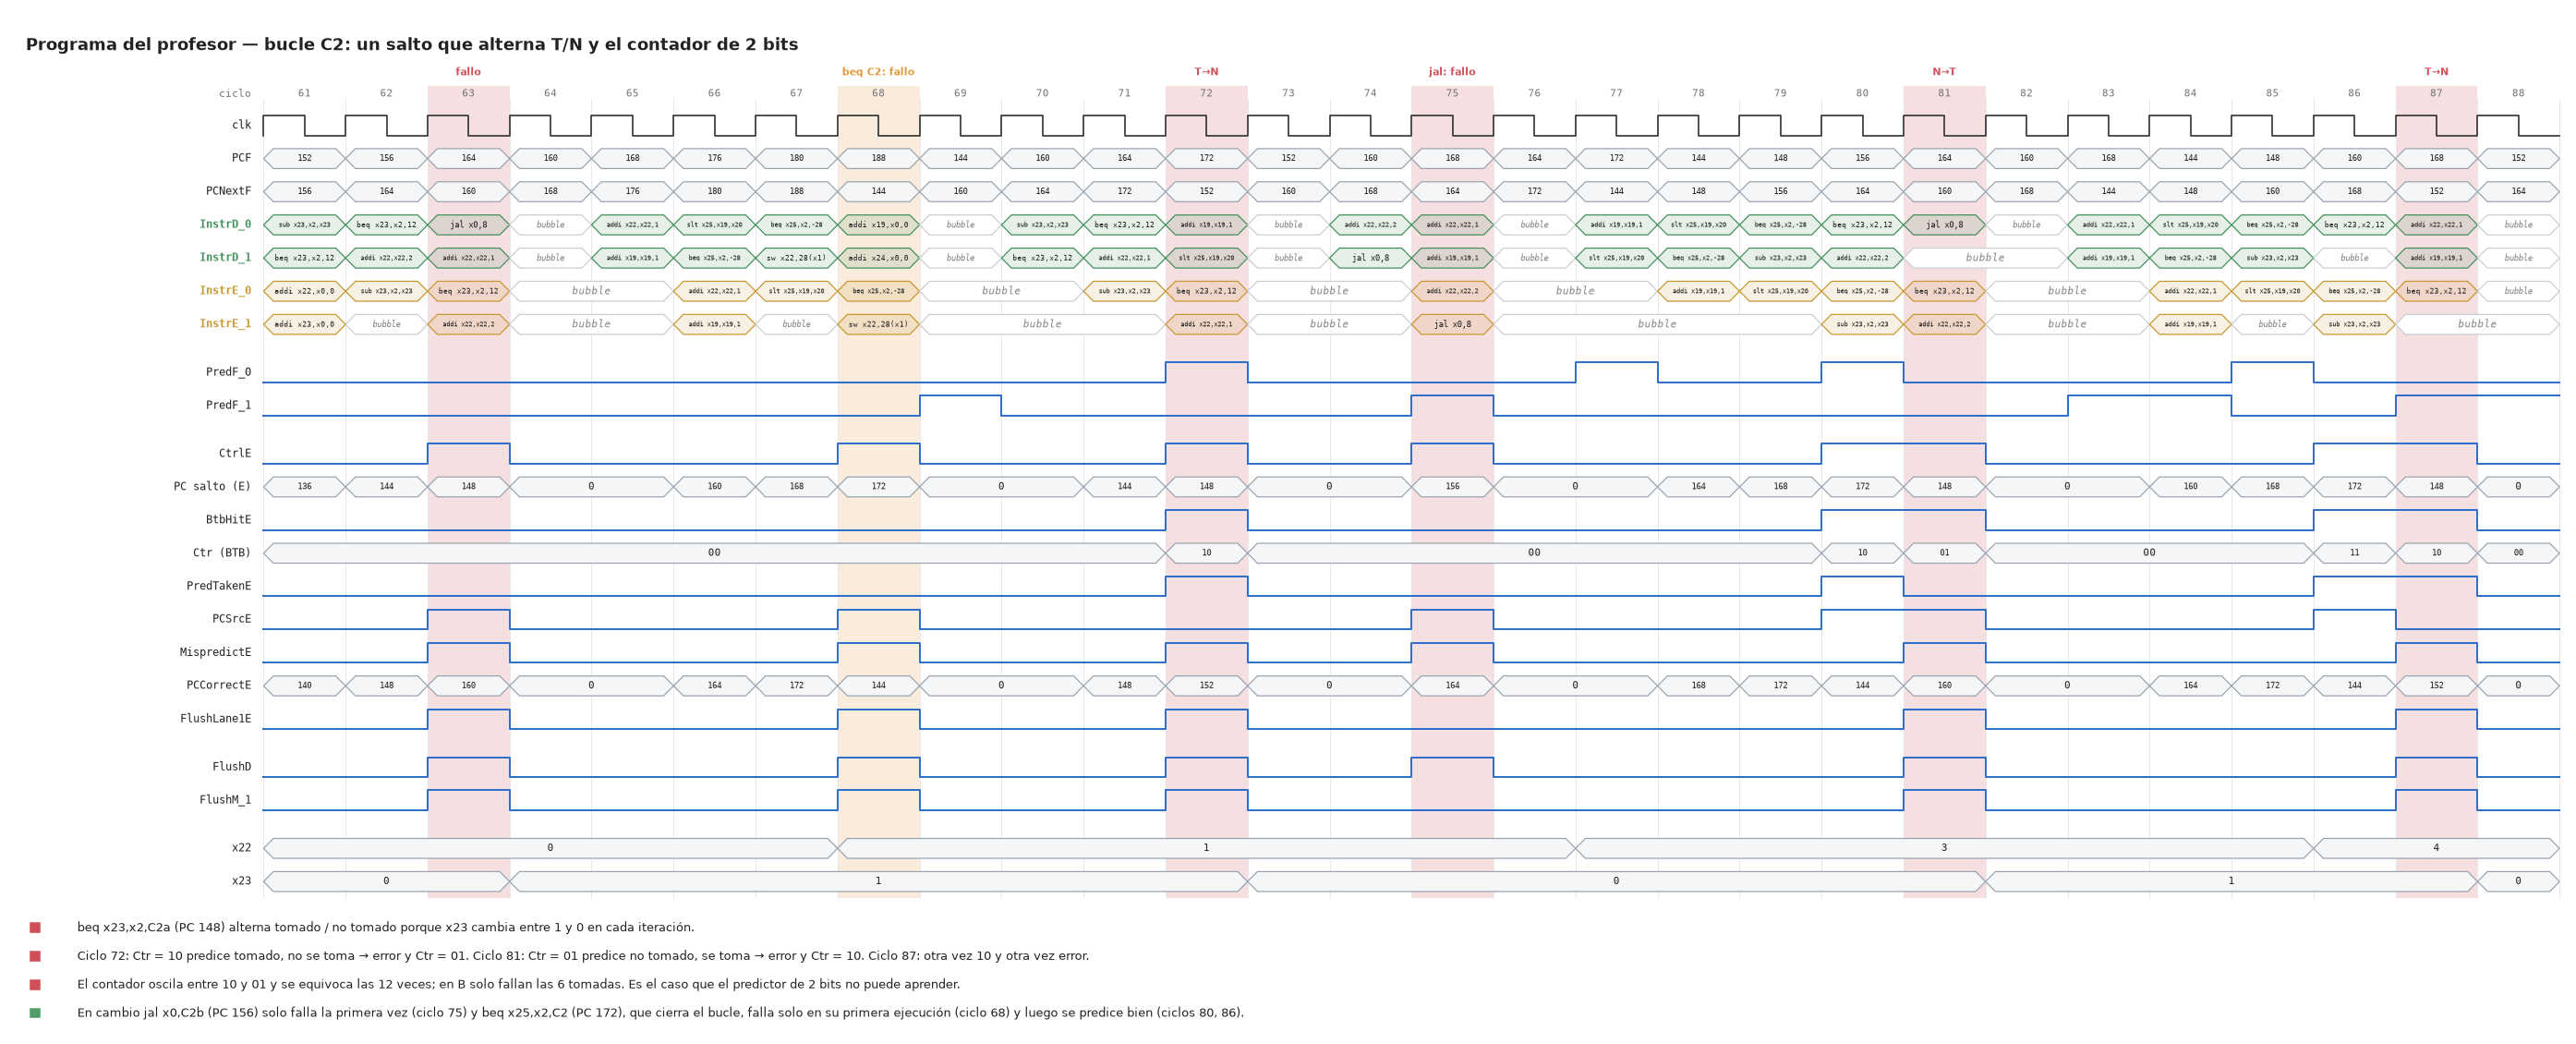
\includegraphics[width=\linewidth,height=0.72\textheight,keepaspectratio]{waveform-prog-C2.png}\par
  \vspace{0.2cm}\small Un salto que alterna (sí, no, sí\ldots). El contador de 2 bits falla \textbf{todas} las veces; B falla solo la mitad.
\end{frame}

\begin{frame}{Resultados de los dos programas}
  \footnotesize
  \centering
  \setlength{\tabcolsep}{5pt}\renewcommand{\arraystretch}{1.2}
  \begin{tabular}{@{}lcccccc@{}}
    \toprule
    & \multicolumn{3}{c}{\textbf{Programa del profesor}} & \multicolumn{3}{c}{\textbf{Programa propio (\textit{bubble sort})}}\\
    \cmidrule(lr){2-4}\cmidrule(lr){5-7}
    \textbf{Indicador} & \textbf{A: Pipeline} & \textbf{B: Dual} & \textbf{C: Dual+BTB} & \textbf{A: Pipeline} & \textbf{B: Dual} & \textbf{C: Dual+BTB}\\
    \midrule
    Ciclos totales & 459 & 387 & \textbf{292} & 1735 & 1421 & \textbf{1163}\\
    Instrucciones retiradas & 312 & 312 & 312 & 1335 & 1335 & 1335\\
    CPI & 1.471 & 1.240 & \textbf{0.936} & 1.300 & 1.064 & \textbf{0.871}\\
    IPC & 0.680 & 0.806 & \textbf{1.068} & 0.769 & 0.939 & \textbf{1.148}\\
    Speedup vs. pipeline & 1.00 & 1.186 & \textbf{1.572} & 1.00 & 1.221 & \textbf{1.492}\\
    Speedup vs. Dual-Issue & --- & 1.00 & \textbf{1.325} & --- & 1.00 & \textbf{1.222}\\
    \midrule
    Errores de predicción & 68 & 68 & 33 & 199 & 199 & 76\\
    Precisión de predicción & 24.4\,\% & 24.4\,\% & 63.3\,\% & 28.7\,\% & 28.7\,\% & 72.8\,\%\\
    \bottomrule
  \end{tabular}
  \vspace{0.1cm}

  \raggedright
  {\tiny\color{muted}Mismo testbench, mismos \texttt{.mem} y mismo periodo de reloj; en el programa del profesor se excluye el bucle \texttt{fin}.}
\end{frame}

\begin{frame}{Análisis: origen de la mejora e IPC lejos de 2}
  \begin{columns}[T]
    \column{0.48\textwidth}
    \textbf{B frente a A}
    \begin{itemize}
      \item Gana en los ciclos en que entran dos instrucciones juntas.
    \end{itemize}
    \medskip
    \textbf{C frente a B}
    \begin{itemize}
      \item Casi toda la diferencia: cada error evitado ahorra \textbf{2 ciclos} de flush.
      \item Entran menos instrucciones del camino incorrecto.
    \end{itemize}
    \column{0.5\textwidth}
    \textbf{Lo que separa a C del IPC ideal de 2}
    \begin{itemize}
      \item \textbf{RAW dentro del par}: \texttt{slt} $\to$ \texttt{beq} en todos los bucles.
      \item \textbf{Un solo puerto de memoria}: los dos \texttt{lw} nunca van juntos.
      \item \textbf{Errores restantes} de predicción.
      \item \textbf{Slot 1 anulado} tras un salto predicho en el slot 0.
    \end{itemize}
  \end{columns}
\end{frame}

\begin{frame}{¿Cuándo es útil la predicción?}
  \begin{columns}[T]
    \column{0.52\textwidth}
    \footnotesize
    \setlength{\tabcolsep}{4pt}
    \begin{tabular}{@{}lcccc@{}}
      \toprule
      \textbf{Salto} & \textbf{Ejec.} & \textbf{Tom.} & \textbf{Err. B} & \textbf{Err. C}\\
      \midrule
      \multicolumn{5}{@{}l}{\textit{Programa del profesor}}\\
      Cierre de C1, C2, C3 (c/u) & 12 & 11 & 11 & \textcolor{good}{\textbf{2}}\\
      \texttt{jal} de C2, C3 (c/u) & 6 & 6 & 6 & \textcolor{good}{\textbf{1}}\\
      C3a (6 T, luego 6 N) & 12 & 6 & 6 & \textcolor{good}{\textbf{3}}\\
      C2a (alterna) & 12 & 6 & 6 & \textcolor{bad}{\textbf{12}}\\
      D2 (según los datos) & 6 & 2 & 2 & \textcolor{bad}{\textbf{4}}\\
      \midrule
      \multicolumn{5}{@{}l}{\textit{Programa propio}}\\
      \texttt{inner} (cierre) & 120 & 105 & 105 & \textcolor{good}{\textbf{16}}\\
      \texttt{noswap} (según los datos) & 120 & 58 & 58 & 53\\
      \bottomrule
    \end{tabular}
    \column{0.46\textwidth}
    \small
    \begin{itemize}
      \item \textcolor{good}{\textbf{Útil}}: cierres de bucle y \texttt{jal}.
      \item \textbf{Parcial}: patrones con pocos cambios (C3a).
      \item \textcolor{bad}{\textbf{Perjudicial}}: saltos que alternan (C2a).
      \item \textbf{Casi nulo}: saltos según los datos (\texttt{noswap}).
      \item \textbf{Sin efecto}: saltos que se ejecutan una sola vez.
    \end{itemize}
  \end{columns}
\end{frame}

% =====================================================================
\section{Conclusiones}

\begin{frame}{Limitaciones, dificultades y mejoras futuras}
  \begin{columns}[T]
    \column{0.32\textwidth}
    \textbf{Limitaciones}
    \begin{itemize}\small
      \item Un error sigue costando 2 ciclos.
      \item La primera vez, todo salto se predice ``no tomado''.
      \item Fetch más largo; no se sintetizó.
    \end{itemize}
    \column{0.32\textwidth}
    \textbf{Dificultades}
    \begin{itemize}\small
      \item Elegir el PC siguiente entre predicción y reagrupamiento.
      \item Que la predicción viaje con su instrucción al reagrupar.
      \item Medir igual en A, B y C.
    \end{itemize}
    \column{0.32\textwidth}
    \textbf{Mejoras futuras}
    \begin{itemize}\small
      \item Predictor con historia para saltos que alternan.
      \item Resolver \texttt{jal} en Decode.
      \item \emph{Instruction Queue}.
    \end{itemize}
  \end{columns}
\end{frame}

\begin{frame}{Conclusiones}
  \begin{itemize}
    \item Dual-Issue In-Order funcional, con recursos compartidos y reagrupamiento.
    \item Las tres arquitecturas dan el mismo resultado en los 23 programas.
    \item Con el BTB: IPC por encima de 1 y $\approx$1.5$\times$ más rápido que el pipeline.
    \item La mejora viene de los saltos que dejamos de fallar, sobre todo en bucles.
    \item No llegamos a IPC 2 por dependencias dentro del par y un solo puerto de memoria.
  \end{itemize}
\end{frame}

\begin{frame}{Reflexión final: ¿cuánto cuesta el paralelismo?}
  \begin{itemize}
    \item \textbf{Dual-Issue}: datapath duplicado (2 ALU, RF 4R/2W, Issue Unit) para $\approx$20\,\% de mejora.
    \item \textbf{BTB}: $\approx$1 Kbit extra, lo mismo que una caché pequeña, para otro 20--30\,\%.
    \item En total $\approx$\textbf{1.5$\times$} más rápido, con bastante más hardware, costo y consumo.
  \end{itemize}
\end{frame}

\begin{frame}[plain,noframenumbering]
  \centering\vfill
  {\color{accent}\Huge\bfseries ¡Gracias!}\par\vspace{0.4cm}
  {\large Preguntas}\par\vspace{0.8cm}
  
\includegraphics[height=1.6cm]{utec-logo.png}
  \vfill
\end{frame}

\end{document}
